\PassOptionsToPackage{final}{graphics}
\PassOptionsToPackage{unicode,pdfencoding=auto}{hyperref}
\def\sectionautorefname{Section}
\def\subsectionautorefname{Section}
\def\subsubsectionautorefname{Section}
\def\tableautorefname{Table}
\def\figureautorefname{Figure}

\documentclass[natbib]{sigplanconf}

 % common/config
\usepackage{fix-cm}
\usepackage[utf8]{inputenc}
\usepackage[T1]{fontenc}
\usepackage[final]{microtype}[2011/08/18]
\usepackage{textcomp}

\setlength{\pdfpageheight}{\paperheight}
\setlength{\pdfpagewidth}{\paperwidth}

\usepackage{ifdraft}

\usepackage{graphicx}
\usepackage{ifthen}
\usepackage{tabularx}
\usepackage{fancyvrb}
\usepackage{xspace}
\usepackage{relsize}
\usepackage{setspace}
\usepackage{booktabs}
\usepackage{natbib}
\usepackage[binary-units]{siunitx}
\usepackage{acronym}
\usepackage{rotating}

\usepackage[final]{listings}

\usepackage{color}
\usepackage[table,svgnames]{xcolor}
\usepackage{newtxmath}
\usepackage[%
  obeyDraft,%
  colorinlistoftodos,%
]{todonotes}

\newcommand\todoauthor[2][\empty]{
  \expandafter\newcommand\csname #2\endcsname[2][\empty]{%
    }}

\def\todosec{\par\noindent\todo[inline]}
\def\secmissing{\par\noindent\todo[color=red,inline,size=\Large]}
\long\def\todolist#1#2{%
\par\noindent%
\todo[inline,color={red!100!green!50},caption={#1}]{%
\begin{minipage}{\linewidth}%
\begin{itemize}
#2%
\end{itemize}
\end{minipage}
}%
}
\ifdraft{%
  \usepackage{blindtext}
  \errorcontextlines=999
  \usepackage{eso-pic}
  \providecommand*\draftFont{\sffamily}
  \newsavebox{\draftPageLine}
  \AddToShipoutPicture{%
    \put(\LenToUnit{-\hoffset},\LenToUnit{\dimexpr\paperheight+\voffset\relax}){%
      \raisebox{-\height}[\height][0pt]{\usebox{\draftPageLine}}}%
    \put(\LenToUnit{-\hoffset},\LenToUnit{\dimexpr\voffset\relax}){%
      \raisebox{\depth}[\height][0pt]{\usebox{\draftPageLine}}}%
  }
  \AtBeginDocument{
    \def\draftInfo{%
      {\draftFont
      Draft Draft Draft%
      \hspace*{5cm}\today\hspace*{5cm}%
      Draft Draft Draft%
      }}
    \sbox{\draftPageLine}{%
      \colorbox{black!10}{%
        \raisebox{0pt}%
        [\dimexpr .33\baselineskip + \height]%
        [\dimexpr .33\baselineskip + \depth]{%
          \makebox[8.5in]{\color{black!50}\draftInfo}}}}
  }
  \AtEndDocument{\listoftodos}
}{
  \let\blindtext\relax
  \let\Blindtext\relax
  \let\blinddocument\relax
  \let\Blinddocument\relax
}

\lstset{%
  basicstyle=\footnotesize\ttfamily,
  columns=fullflexible,
  captionpos=b,
  floatplacement=htbp,
  upquote=true,
  numbers=left, numberstyle=\tiny\color{black!33},numbersep=5pt}
\AtBeginDocument{
  \lstMakeShortInline[language=JavaScript]|
}
\usepackage[%
  final, pdfpagelabels=false,
  hidelinks, %
  plainpages=true,%
]{hyperref}

\providecommand*{\lstnumberautorefname}{line}
\providecommand*{\lstlistingautorefname}{listing}
\renewcommand*{\subsectionautorefname}{section}

\newcommand*\hairspace{\ifmmode\mskip1mu\else\kern0.08em\fi}
\iffalse
\newcommand*{\eg}{e.\hairspace{}g.\xspace}
\newcommand*{\Eg}{E.\hairspace{}g.\xspace}
\newcommand*{\Ie}{I.\hairspace{}e.\xspace}
\newcommand*{\ie}{i.\hairspace{}e.\xspace}
\else
\newcommand*{\eg}{e.\hairspace{}g.,\xspace}
\newcommand*{\Eg}{E.\hairspace{}g.,\xspace}
\newcommand*{\Ie}{I.\hairspace{}e.,\xspace}
\newcommand*{\ie}{i.\hairspace{}e.,\xspace}
\fi

\lstset{language=JavaScript}

\todoauthor[teal]{topa}
\todoauthor[lime]{tim}
\todoauthor[violet!50]{bert}
\todoauthor[purple]{rhi}
\todoauthor[yellow]{dan}

\newcommand*\SqueakJS{Squeak\texorpdfstring{\kern.04em}{}JS\xspace}
\newcommand*\SqueakST{Squeak\kern.1em /\kern.1em\penalty0 Smalltalk\xspace}
\newcommand*\JS{JavaScript\xspace}
\newcommand*\RSqueakVM{R\kern.05em /\kern.02em Squeak\kern-.1emVM\xspace}
\newcommand*\IndexedDB{\mbox{Indexed\kern.05em DB}\xspace}

\newcommand*\SqueakJSTitle{\SqueakJS}
\newcommand*\SqueakJSSubtitle{A Modern and Practical Smalltalk that Runs in Any Browser}
\newcommand*\SqueakJSKeywords{Smalltalk, Squeak, Web browsers, \JS}

\hypersetup{
  pdfsubject={DLS'14},
  pdfkeywords={\SqueakJSKeywords},
  pdftitle={\SqueakJSTitle: \SqueakJSSubtitle},%
    pdfauthor={%
      Bert Freudenberg,
      Dan Ingalls,
      Tim Felgentreff,
      Tobias Pape,
      Robert Hirschfeld}}

\nocaptionrule

\titlebanner{preprint --- SqueakJS --- preprint}
\preprintfooter{SqueakJS}

\usepackage{fixltx2e}

\begin{document}

\exclusivelicense
\conferenceinfo{DLS~'14}{October 20--24, 2014, Portland, OR, USA}
\copyrightyear{2014}
\copyrightdata{978-1-4503-3211-8/14/10}
\doi{10.1145/2661088.2661100 }

\newacro{JIT}[\textsc{jit}]{just-in-time}
\newacro{API}[\textsc{api}]{application programming interface}
\newacro{AST}[\textsc{ast}]{abstract syntax tree}
\newacro{VM}[\textsc{vm}]{virtual machine}
\newacro{GC}[\textsc{gc}]{garbage collection}
\newacro{DOM}[\textsc{dom}]{document object model}
\newacro{ID}[\textsc{id}]{identifier}
\title{\SqueakJSTitle}
\subtitle{\SqueakJSSubtitle}

\authorinfo{Bert~Freudenberg}
           {Communications Design Group\\Potsdam, Germany}
           {bert@cdglabs.org}
\authorinfo{Dan~Ingalls}
           {Communications Design Group\\San Francisco, CA, USA}
           {dan@cdglabs.org}
\authorinfo{Tim~Felgentreff}
           {Hasso Plattner Institute\\University of Potsdam, Germany}
           {tim.felgentreff@hpi.uni-potsdam.de}
\authorinfo{Tobias~Pape}
           {Hasso Plattner Institute\\University of Potsdam, Germany}
           {tobias.pape@hpi.uni-potsdam.de}
\authorinfo{Robert~Hirschfeld}
           {Hasso Plattner Institute\\University of Potsdam, Germany}
           {robert.hirschfeld@hpi.uni-potsdam.de}

\maketitle

\begin{abstract}
  We report our experience in implementing \SqueakJS, a bit-compatible
  implementation of \SqueakST written in pure \JS. \SqueakJS runs
  entirely in the Web browser with a virtual file system that can be
  directed to a server or client-side storage. Our implementation is
  notable for simplicity and performance gained through adaptation to
  the host object memory and deployment leverage gained through the
  Lively Web development environment. We present several novel
  techniques as well as performance measurements for the resulting
  virtual machine. Much of this experience is potentially relevant to
  preserving other dynamic language systems and making them available
  in a browser-based environment.
\end{abstract}

\category{D.3.4}{Software}{Programming Languages}[Interpreters]
\terms
Languages, Virtual Machines, Performance
\keywords
\SqueakJSKeywords

\section{Motivation}

The \SqueakST development
environment~\cite{IngallsKaehlerMaloneyWallaceKay97} and its
derivatives are the basis for a number of interesting applications in
research and education. Educational applications such as Etoys
\cite{Kay05} and early versions of Scratch \cite{maloney2004scratch},
however, suffer from restrictions against installing native software
in scholastic environments. To cope with this limitation, web browsers
have become the preferred target for those applications; Scratch has
been rewritten in Flash, and for Etoys, a browser plugin for major web
browser has been available for a several years. Yet, both approaches
still need either software alien to the browser or a complete
rewrite. With \JS as the de-facto standard for Web programming, a
\JS-based, and thus browser-native, implementation of Squeak's \ac{VM}
is desirable.

\begin{figure}
  \centering
  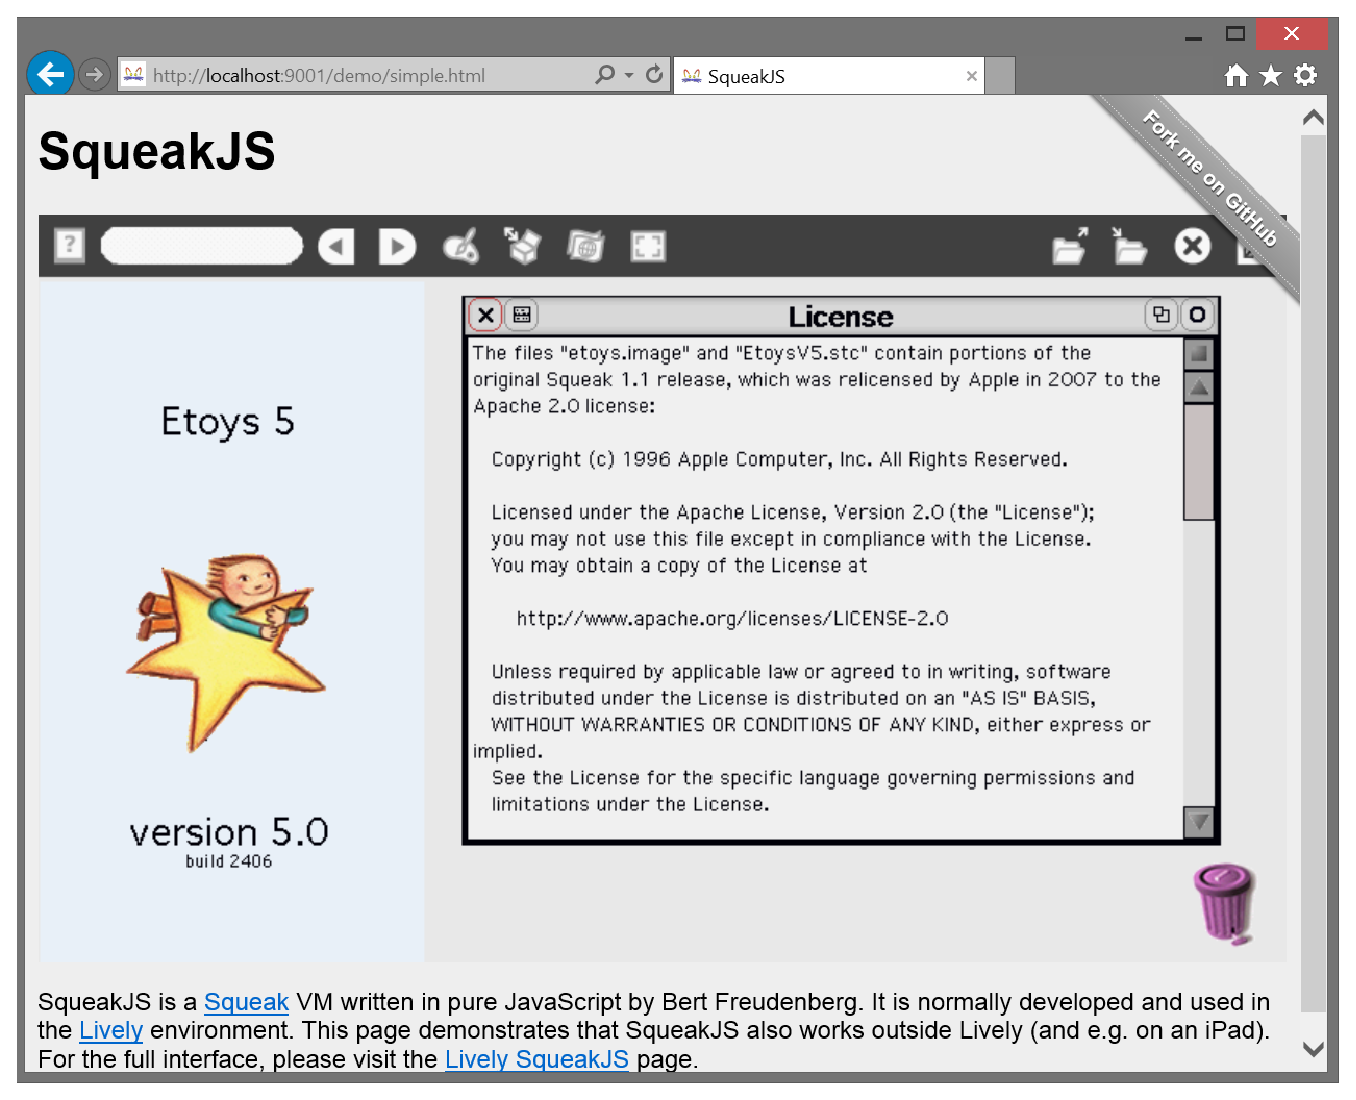
\includegraphics[width=\linewidth]{squeakjs-running}
  \caption{\SqueakJS running an Etoys image in a stand-alone Web page}
  \label{fig:squeakjs}
\end{figure}

With \SqueakJS, we aim to provide a fully backwards-compatible
\SqueakST system in the browser, able to directly run applications
like Etoys or Scratch. \autoref{fig:squeakjs} shows \SqueakJS running
a Squeak Etoys image directly in the browser\footnote{Squeak images
  are binary dumps of a running Squeak system's memory. \SqueakJS
  supports reading and writing the same format as the standard Squeak
  \ac{VM}.}, on a plain HTML page.

Dynamic languages such as Python or Ruby have successfully been
translated into \JS using the automatic translation tool-chain
Emscripten~\cite{Zakai11}. In contrast to such language
implementations that host much of its core functionality inside of the
\ac{VM}, Squeak implements much of its kernel in
Smalltalk~\cite{GoldbergRobson83} itself. Additionally, Squeak is a
graphical programming system and, to run in the browser, requires at
least minimal interaction with the browser's \ac{DOM}.

Recent attempts at re-implementing or re-engineering the Squeak
\ac{VM} have shown that good performance is difficult to achieve
\cite{Bolz+2008:Back-to-the-Future-in-One-Week,marr2012identifying,Wassermann13}. To
us, Squeak appeared to be too slow to actually emulate in \JS, and too
complex to subdivide into an interpreter layer and browser graphics
layer.

Potato, an earlier Squeak \ac{VM} experiment written in Java, allowed
us to asses the performance of our approach, and served
as basis for the \SqueakJS design in many respects, like the mapping
of Squeak objects to \JS objects or the separation of the
\ac{VM} into the interpreter and a primitive handler.

The fact that \SqueakJS represents Squeak objects as plain \JS
objects and integrates with the \JS \ac{GC} allows existing
\JS code to interact with Squeak objects. This has proven
useful during development as we could re-use existing \JS tools
to inspect and manipulate Squeak objects as they appear in the
\ac{VM}.  This means that \SqueakJS is not only a ``Squeak in the
browser'', but also that it provides practical support for using
Smalltalk in a \JS environment.

In this paper, we report our experience with this implementation,
highlighting the following items in particular:
\begin{itemize}
\item the mapping of Squeak objects in the \ac{VM} to \JS
  objects with direct references,
\item a hybrid garbage collection scheme to allow Squeak object
  enumeration without a dedicated object table, while delegating as
  much work as possible to the \JS \ac{GC},
\item a Web-appropriate adaption of file management to load and store
  Squeak images and other file types supported within Squeak, and
\item the interaction with \JS for clipboard access, graphics,
  debugging, and providing plugins, that allowed us to use a
  rapid-prototyping approach to \ac{VM} development.
\end{itemize}

The rest of this paper is structured as follows: We describe our
rationales for resolving various issues that emerged in our attempt to implement a
Squeak \ac{VM} in the browser. A description of the implementation
details of \SqueakJS, highlighting its innovative approaches, follows in
\autoref{sec:impl}. We evaluate our findings in \autoref{sec:eval} and
put \SqueakJS into perspective with other work in
\autoref{sec:related}. Finally, \autoref{sec:conclusion} presents some
lessons learned and suggestions for future work.

\section{Approach}
\label{sec:approach}

The core of \SqueakJS is inspired by Potato, a Squeak \ac{VM} written
in Java. The sources of its precursor, Dan Ingalls's 2008 original ``JSqueak'',
served as reference. Some fundamental design decisions, such as the mapping of Squeak
objects to \JS objects or the separation of the VM into the interpreter
and a primitive handler are exactly as in Potato. Some parts of the
interpreter were transcribed literally, just removing Java's type
annotations. Even some bugs were faithfully transcribed and only fixed later.

Apart from using another programming language, there are also differences in the
\SqueakJS implementation. For example, there is no object table,
corresponding to the WeakReference array that is used in Potato for
object enumeration.

These implementation differences, however, are less important than the
context for which \SqueakJS is intended. Java applications are less
accommodating to direct manipulation development than \JS applications
where live objects are inspected and manipulated with developer tools
at run-time. Besides Browser-provided introspection tools,
self-supporting development environments in the browser such as the
Lively Kernel provide developers with malleable tools that can be
easily adapted for specific use-cases. In Lively, most tools are
\emph{parts}~\cite{lincke2012lively}---parts are compositions of
\emph{morphs}~\cite{maloney1995morphic} with associated,
instance-specific behavior. In this context, the properties inherited
from Potato are beneficial and allowed us to tailor Lively's tools
towards inspecting and debugging the \ac{VM} to provide immediate
feedback during the development of \SqueakJS.

\subsection{Getting it Going}
\label{sec:getting-it-going}

Squeak has been implemented a number of times by now. The
process to get it up and running roughly consists of the steps
described by Dan Ingalls~\cite{IngallsKaehlerMaloneyWallaceKay97}:

\begin{itemize}
\item implement a new image reader and writer,
\item write a new interpreter and essential plugins such as BitBlt
and FilePlugin, and
\item compile the interpreter to make it practical.
\end{itemize}

Of these steps, only the first two apply to our context. We decided
early on to transcribe our implementation from the Potato sources. The
original Squeak \ac{VM} is written in ``Slang'', a subset of Smalltalk
with C semantics, which can be translated to C
easily~\cite{GuzdialRose02}. It does not use any of C's structured
data types to describe objects. Instead, Slang operates on words in
memory, much like machine code would. The Slang-to-C translator could
be re-targeted to produce Java or \JS, but that would keep these
low-level semantics, which does not map well to a high-level language.
That is why Potato and \SqueakJS are not based on the Slang
implementation.

\begin{figure}
  \centering
  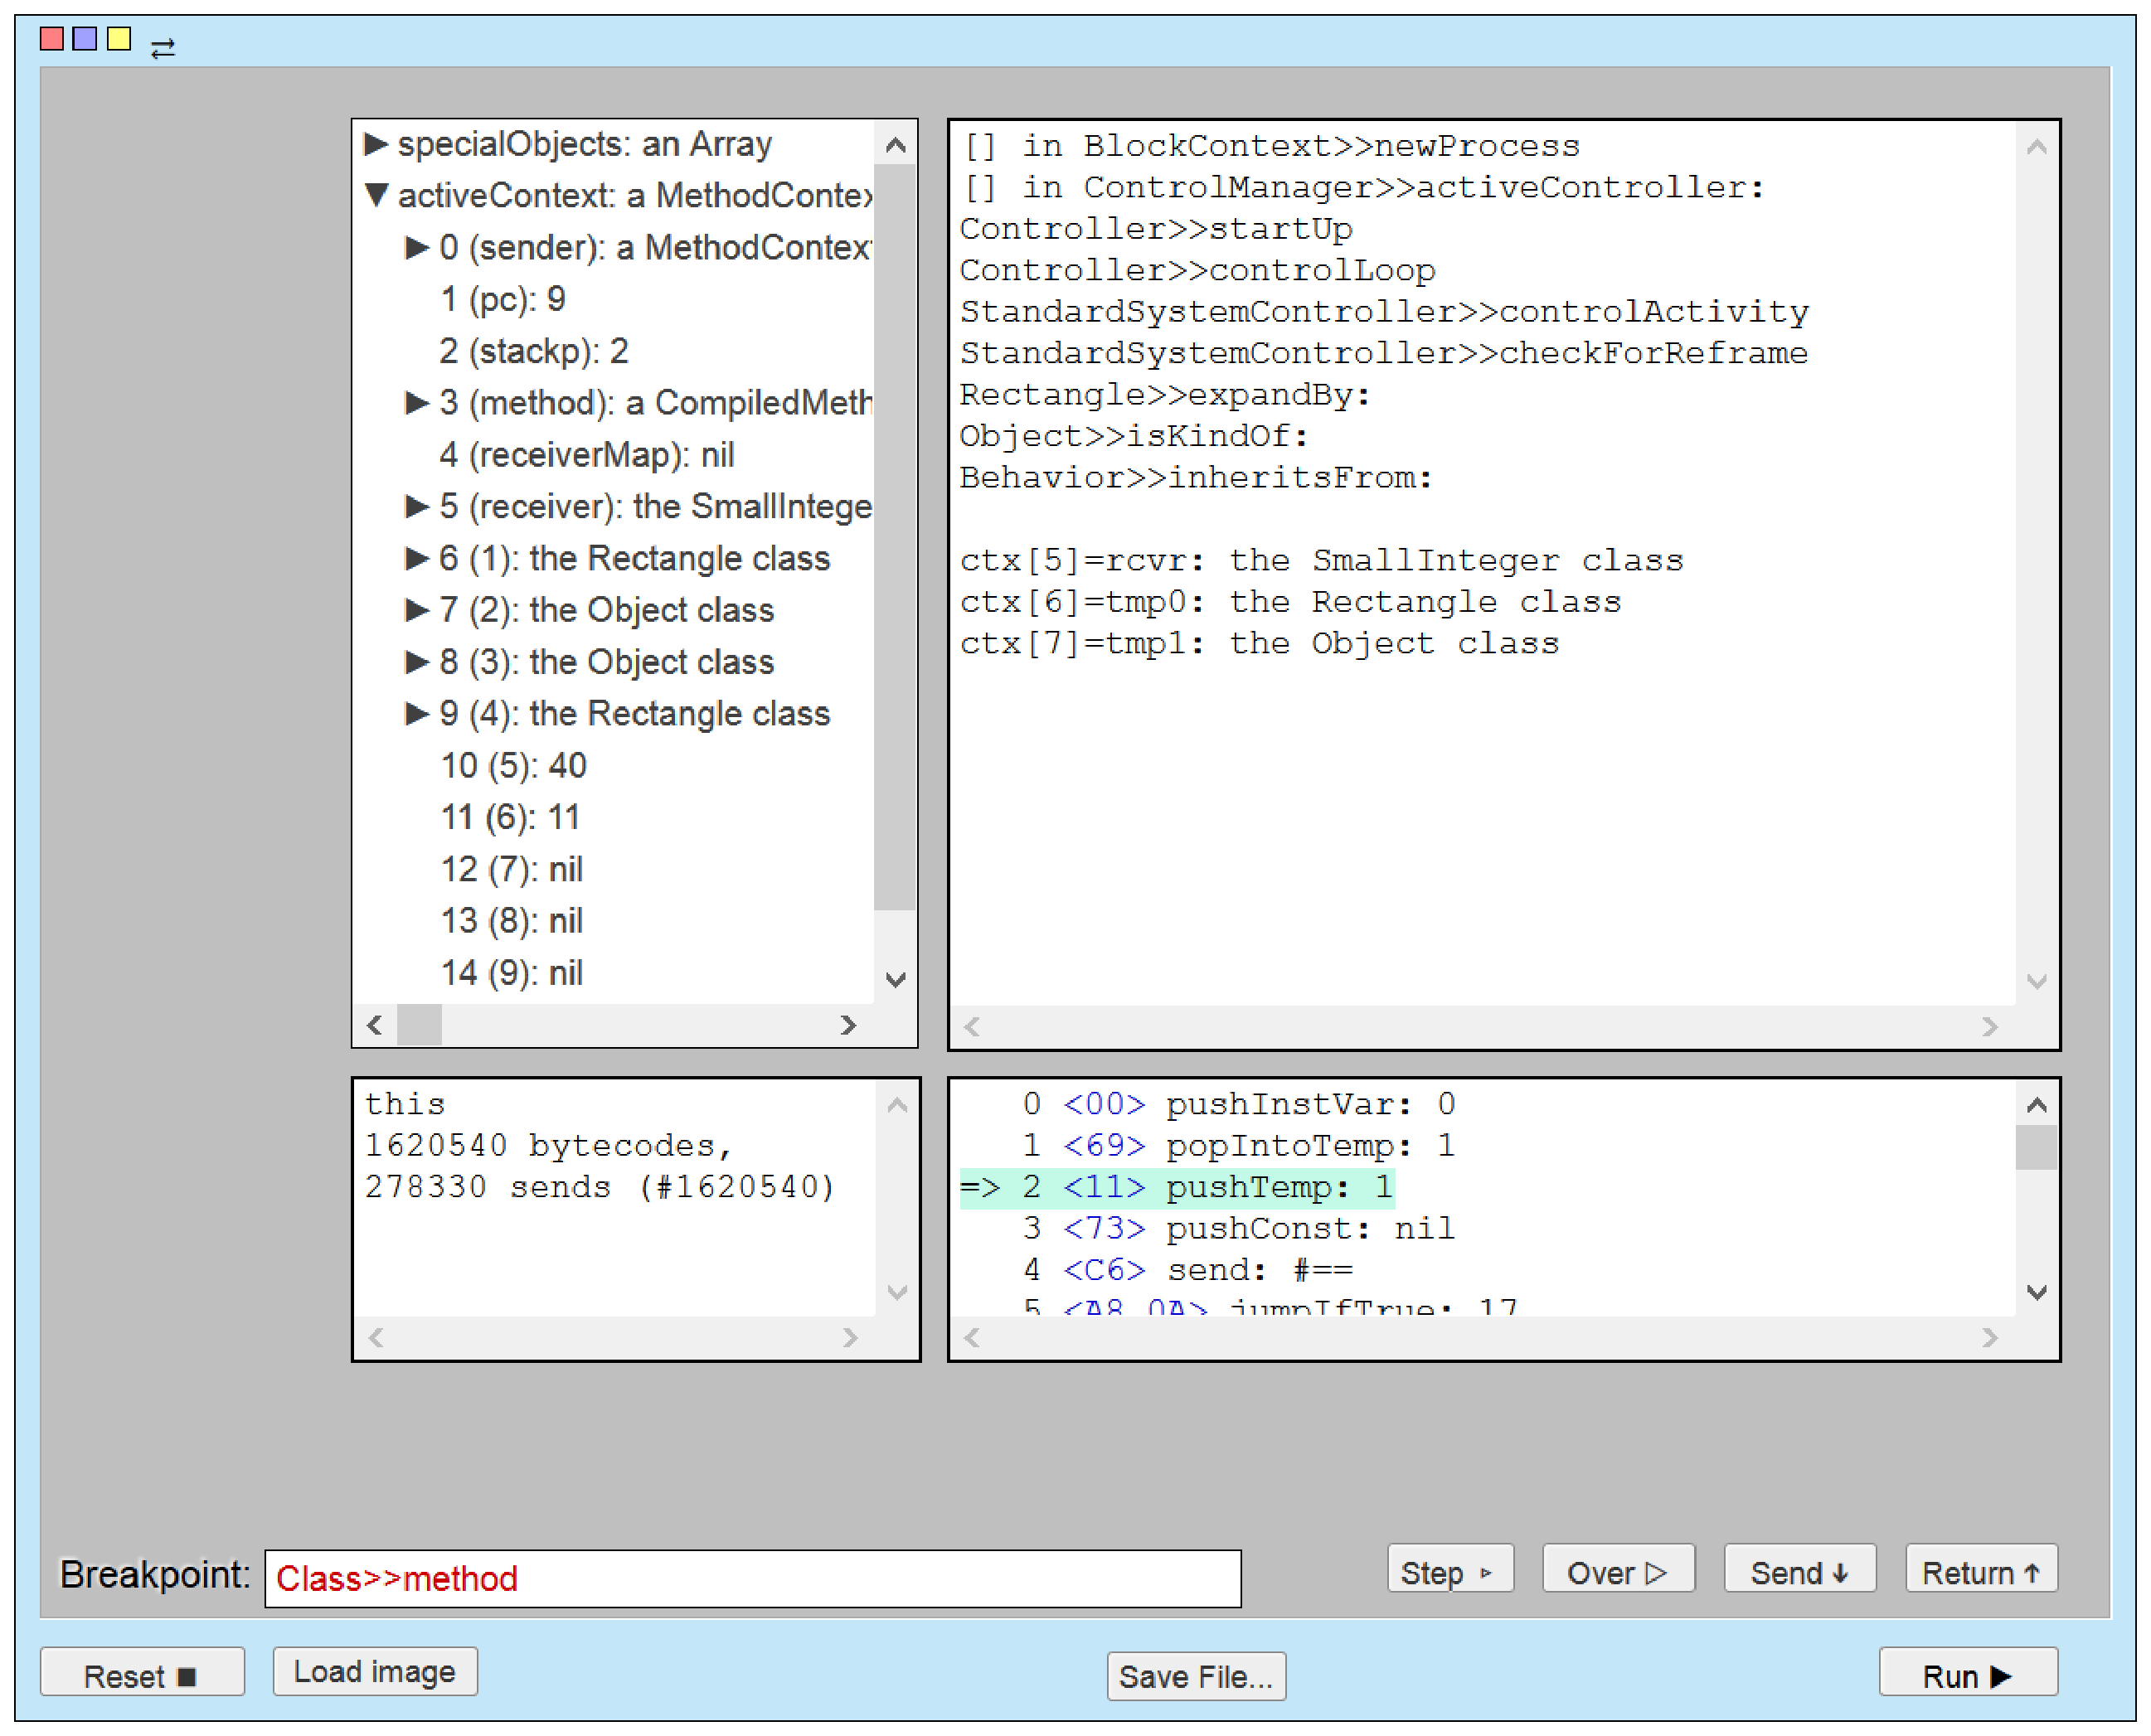
\includegraphics[width=\linewidth]{lively_vm_part}
  \caption{A Lively tool to load Squeak images, inspect, and debug \SqueakJS}
  \label{fig:virtualmachineinspector}
\end{figure}

Potato's object representation departs significantly from that of
Squeak. All Squeak objects appear as plain Java objects, with slots
that store the information required by the \ac{VM} such as instance
variables, class, format code, and indexable data. The same scheme is
carried forward in \SqueakJS.  In the context of Lively, this allows
us to easily adapt existing \JS tools to work on Squeak objects. Once
the image loader began working, we could compose various Lively tools
to create a virtual machine inspector, as shown in
\autoref{fig:virtualmachineinspector}.

Because stack frames and threads (contexts and processes in Squeak
parlance) are Squeak objects as well, we can use the inspector to
watch the \ac{VM} stack while it is executing and debug any problems
directly. This was useful early on to verify that the image loader and
scheduler work correctly, and that dispatch actually worked when the
\ac{VM} started executing. Additionally, the debugging support
available in Squeak---to break at, step into, and to disassemble
methods---is available to the inspector as well.

\subsection{Drawing to the Screen}
Besides the interpreter, some way of drawing to the screen is
required. Squeak uses a BitBlt plugin to render into bitmaps, which is
fairly well separated from the rest of the interpreter. Potato only
supports \SI{1}{\bit} per pixel color depths and a minimal set of
graphics features. To support full color and all graphics features
used in modern Squeak and Etoys image, the much larger Slang code for
the BitBlt and WarpBlt plugins had to be transcribed to \JS.

Both BitBlt and WarpBlt can be simulated in Squeak, so conceivably,
the Smalltalk code could be executed directly to render graphics. The
\RSqueakVM (based on the Spy%
~\cite{Bolz+2008:Back-to-the-Future-in-One-Week}) is an RPython-based
implementation of Squeak that uses this scheme \cite{Wassermann13}.
However, even with RPython's tracing \ac{JIT} compiler~\cite{Bolz12},
the performance of pure-Smalltalk BitBlt is still about an order of
magnitude slower than a C-based implementation, indicating that a
native (which in our case means \JS) implementation is still
preferable to achieve good performance.

\SqueakJS exposes a module interface similar to that of regular Squeak
\acp{VM}, and BitBlt is implemented as an internal module, i.\,e., one
that comes with the \ac{VM}. A simple HTML5 canvas is used to mirror
the contents of the Squeak display object, a bitmap object that
contains an array of bytes. Whenever an update to the display is
needed, the Squeak system calls a primitive, which we use to update
the HTML5 canvas.

Another module required by modern Squeak images is the ``Balloon'' 2D
renderer. It supports anti-aliased drawing of graphics primitives not
available in BitBlt, \eg Bézier curves (needed to render
True\kern-.05em Type fonts), and color gradients (used on various user
interface elements). Porting the Slang code for this module would have
been a major undertaking, likely resulting in a very slow simulation.
Instead, we use an off-screen HTML5 canvas to draw these shapes, read
the pixels back, and composite them over the original Squeak bitmap.

\subsection{Cleaning up Garbage}

Many core functions in Squeak depend on the ability to enumerate
objects of a specific class using the \lstinline{firstInstance} and
\lstinline{nextInstance} primitive methods. In Squeak, this is easily
implemented since all objects are contiguous in memory, so one can
simply scan from the beginning and return the next available instance.
This is not possible in a hosted implementation where the host does
not provide enumeration, as is the case for Java and \JS. Potato used
a weak-key object table to keep track of objects to enumerate them.
Other implementations, like the \RSqueakVM, use the host
garbage collector to trigger a full \ac{GC} and yield all objects of
a certain type. These are then temporarily kept in a list for
enumeration. In \JS, neither weak references, nor access to the
\ac{GC} is generally available, so neither option was possible for
\SqueakJS. Instead, we designed a hybrid \ac{GC} scheme that provides
enumeration while not requiring weak pointer support, and still
retaining the benefit of the native host \ac{GC}.

\SqueakJS manages objects in an \emph{old} and \emph{new} space, akin
to a semi-space \ac{GC}. When an image is loaded, all objects are
created in the old space. Because an image is just a snapshot of the
object memory when it was saved, all objects are consecutive in the
image. When we convert them into \JS objects, we create a
linked list of all objects. This means, that as long as an object is
in the \SqueakJS old-space, it cannot be garbage collected by the
\JS \ac{VM}. New objects are created in a virtual \emph{new}
space. However, this space does not really exist for the \SqueakJS
\ac{VM}, because it simply consists of Squeak objects that are not
part of the old-space linked list. New objects that are dereferenced
are simply collected by the \JS \ac{GC}.

When full \ac{GC} is triggered in \SqueakJS (for example because the
\lstinline{nextInstance} primitive has been called on an object that
does not have a next link) a two-phase collection is started. In the
first pass, any new objects that are referenced from surviving objects
are added to the end of the linked list, and thus become part of the
\emph{old} space. In a second pass, any objects that are already in
the linked list, but were not referenced from surviving objects are
removed from the list, and thus become eligible for ordinary
\JS \ac{GC}. Note also, that we append objects to the old list
in the order of their creation, simply by ordering them by their
object \acp{ID}. In Squeak, these are the memory offsets of the object. To
be able to save images that can again be opened with the standard
Squeak \ac{VM}, we generate object \acp{ID} that correspond to the offset
the object would have in an image. This way, we can serialize our old
object space and thus save binary compatible Squeak images from
\SqueakJS.

To implement Squeak's weak references, a similar scheme can be
employed: any weak container is simply added to a special list of root
objects that do not let their references survive. If, during a full
\ac{GC}, a Squeak object is found to be only referenced from one of
those weak roots, that reference is removed, and the Squeak object is
again garbage collected by the \JS \ac{GC}.

\subsection{Adapting Squeak for the Web}
\label{sec:adapting-for-web}

A general problem when running Squeak in a Web browser is the
asynchronous nature of \JS. While most \acp{VM} are implemented as a
main loop that simply executes until the \ac{VM} is stopped, \SqueakJS
needs access to input events that are generated by the browser, and
has to give the browser time to update the \ac{DOM}. Our solution to
this problem is to have \SqueakJS regularly break out of its
interpreter loop and schedule a timeout function to continue running
after events have been processed.

Another common problem of running \JS applications is the question of
file system access. While Squeak can work without a file system, a lot
of functionality would be missing without the ability to store
files. This presents a challenge for a system designed to run in a
browser. One option would be to upload files to and retrieve them from
a server. But this would require continuous connectivity, and we want
\SqueakJS to be usable offline.

Three options are available to store data in a browser. The first is
browser cookies, on top these, simple key-value stores can be
implemented. However, cookies are limited to \SI{4}{\kilo\byte} and
are not a good fit to emulate a file system, considering that to save
a modern Squeak image requires from ten to hundreds of Megabytes. The
second option is the browser's local storage \cite{hickson2013web}.
Like cookies, the amount of local storage per web page is limited, in
most browsers to \SI{5}{\mega\byte}. Again, this prevents us from
saving most modern Squeak images. The third and most recent way to
store files in a browser is \IndexedDB~\cite{mehta2013indexed}.

\IndexedDB is the only viable option that provides enough storage to
be useful as a file system for \SqueakJS. It can store arbitrary \JS
objects and is intended to have both an asynchronous and synchronous
\ac{API}. However, all current implementations only provide the
asynchronous \ac{API}, whereas Squeak expects file system calls to
work synchronously. Breaking out of the interpreter loop as described
previously allows the browser to process asynchronous events. However,
accessing the IndexedDB may take longer than one event loop. To be
able to simulate a synchronous API, we additionally need to be able to
freeze the \ac{VM}---instead of scheduling the next interpretation
step, the main loop simply stores a continuation to continue running
when it is unfrozen. When a file primitive is called, the \ac{VM} is
frozen, and the callback that receives the \IndexedDB unfreezes the
\ac{VM}. The same scheme can be used to synchronize any asynchronous
\JS \ac{API} that we want to expose. This is useful even for network
operations, so that only \SqueakJS, and not the entire browser, waits
for a response.

\section{Implementation}
\label{sec:impl}

Our implementation closely follows the Potato \ac{VM} in its basic
approach, but deviates to accomodate \JS's execution
environment. \SqueakJS is publicly available on
GitHub\footnote{\url{https://github.com/bertfreudenberg/SqueakJS/}}.

\subsection{Object Representation}
\label{sec:objrep}

Implementation of a Smalltalk virtual machine is facilitated by the
relatively clean separation between the byte code interpreter, the
object memory and the graphics system. As noted above, Potato departed
significantly from the Squeak object implementation without
introducing any major perturbations in the rest of the virtual
machine. All Squeak objects were mapped to Java objects with slots for

\begin{itemize}
\item Squeak hash (short)
\item Squeak format code (short)
\item class (pointer)
\item pointer fields (array of pointers for instance variables and indexable fields)
\item indexable binary data fields (array of bytes or ints)
\end{itemize}

As the only exception, SmallIntegers were represented by Java
\lstinline|Integer| objects. This is similar to the tagged pointers in
other Squeak \acp{VM} which are used to represent immediate SmallInteger
values. In contrast, Floats are represented by full objects, but their
binary data slot was set to a Java \lstinline|Double| so it could be
accessed more quickly in arithmetic primitives.

Essentially the same scheme is used in \SqueakJS. Since the layout of \JS
objects does not have to be declared in advance, slots are added only when
needed. The pointers (instance variables and indexable fields), words, and
bytes slots are only present if the object actually needs them, that is, there
is at least one element. We chose an array for storing instance variables
rather than named \JS properties because the bytecodes reference them by
index, not by name. SmallIntegers are directly represented by \JS numbers. In
places where the \ac{VM} needs to distinguish SmallIntegers from other objects it
uses a \lstinline|typeof| check.

For making common tests more efficient, \SqueakJS also adds flags to special
objects. For example, the \lstinline|isNil| property is added to the
\lstinline|nil| object so that a test for being nil can be written without
having to compare it to the \ac{VM}'s \lstinline|nil| object. Floats are marked by
an \lstinline|isFloat| property, and the numeric value is stored directly in
another property. The conversion to words happens on-the-fly, and only when
the image tries to index individual words of the Float object.

In the C implementation, each object was uniquely identified through
its position in memory, exposed to Smalltalk as the \lstinline|oop|
property. \SqueakJS maintains the \lstinline|oop| numeric property
mainly for identifying objects when saving a snapshot. The
\lstinline|oop| also serves as a key when objects need to be added to
a hash map temporarily (\eg during ``become'' operations) because \JS
does not provide an object-keyed hash map. New objects are assigned
consecutive negative oops. A real oop is assigned when the object
survives a full garbage collection, and during compaction oops are
adjusted to account for released objects. This emulates the
consecutive memory layout of the C Squeak \acp{VM} which is manifest in the
snapshot format. The \lstinline|oop| also helps to distinguish objects
while debugging. The essential properties for a Squeak object in
\SqueakJS are thus:

\begin{itemize}
\item hash (\lstinline|number|)
\item format (\lstinline|number|)
\item class (\lstinline|object|)
\item oop (\lstinline|number|)
\item pointers (\lstinline|Array|, optional)
\item words (\lstinline|Uint32Array|, optional)
\item bytes (\lstinline|Uint8Array|, optional)
\item mark (\lstinline|false|, present after surviving \ac{GC})
\item nextObject (\lstinline|object|, present only for objects in old space)
\end{itemize}

The implementation takes advantage of a few \JS idiosyncrasies like treating
a non-existing property as \lstinline|false|. For instance, a newly allocated object
does not have the \lstinline|mark| property, while an old object might have it
set to \lstinline|true| or \lstinline|false| during \ac{GC}. But the test can
simply be written as ``\lstinline|if (obj.mark) ...|'' because both cases test
equally.

\subsection{Object Enumeration and Garbage Collection}

For object enumeration and finding all instances of a class, Squeak uses a
primitive to answer the ``next object'' for a given object, or the next
instance given a particular instance. The next object is easily found since
all objects are contiguous in main memory, so simply adding the size of an
object to the object's address gives the address of the next object. This is
not possible for Potato or \SqueakJS.

Since Java provides no facility for enumerating objects, Potato used
an object table for the sole purpose of enumeration, as required by
Squeak's enumeration facility as well as to support object mutation
which involves enumeration implicitly. By making use of weak pointer
objects in the object table, it was possible to leave the task of
garbage collection entirely up to the Java runtime, a key to that
port. In this regard, it is similar to Hobbes, a \ac{VM} for the
original Smalltalk-80 written for VisualWorks Smalltalk (see
\autoref{sec:dynam-lang-impl}.) Unfortunately, current \JS engines
provide no support for weak pointers. This means that the use of an
object table for enumeration was out of the question, since it would
have prevented all objects from being garbage-collected by the \JS
runtime.

An important innovation in the \SqueakJS object memory is the use of
enumeration links in a subset of Squeak objects that corresponds to
long-lived objects, or what is commonly referred to as ``old space''.
When loading an object snapshot, objects are created as outlined
above.  Additionally, each object is assigned a \lstinline|nextObject|
slot pointing to the next object. The first and last object in this
linked list is held in the VM, constituting the ``old space''. When a
new object is allocated at runtime, it is not added to that list
immediately. Instead, it is only held by references from other objects
and released automatically when no longer referenced.

For old objects that are in the old space linked list, the ``next
object'' primitive can simply return the object's
\lstinline|nextObject|. But for a new object, which does not have the
\lstinline|nextObject| slot yet, a full garbage collection is
triggered. This adds the object (and all other surviving new objects)
to the old-space list, setting the \lstinline|nextObject|, so the
enumeration can continue.

The full \ac{GC} is a variation on mark-and-sweep: In the first phase,
all objects reachable from the roots are marked recursively. If a new
object is found in this phase, it is added to a temporary collection.
In the second phase, the old-space linked list is traversed, unmarked
objects are unlinked, and the mark of remaining objects is cleared.
Finally, the new objects from the first phase are linked to the end of
the old-space list. The discovery of new objects from the ``virtual''
new space during the mark phase is what sets this \ac{GC} apart.

Interestingly, a full garbage collection does not occur regularly as
in most other implementations, since our new space is essentially
unlimited. No objects are tenured outside the full \ac{GC}, so there
is no need to regularly compact old space. In fact, that \ac{GC} is
invoked only from operations that are known to be expensive in the
regular Squeak \ac{VM}: \lstinline|become:|, and
\lstinline|allInstances|\thinspace{}/\thinspace{}\lstinline|allObjects|.
These operations are avoided in general because of their cost, and
hence occur only in code sections that are not critical to
performance. For example, during running the benchmarks in
\autoref{sec:performance} not a single full \ac{GC} happened, even though
about 15 million objects were allocated. In contrast, the startup code
of an Etoys image does 12 \lstinline|allInstances| calls resulting in
as many full \acp{GC}, taking on average \SI{300}{\ms}, tenuring 980 of
150,000 allocated objects. But during normal operation, again, no full
\acp{GC} occur.

\subsection{Snapshotting}

The Potato implementation, being a proof of concept only, did not support
saving object images that could be stored and resumed elsewhere. The \SqueakJS
implementation provides this function in the following manner.

A Squeak object image consists of a file header for basic parameters
followed by a literal memory dump of the object memory. Objects are
laid out consecutively, with each object consisting of one to three
header words followed by zero or more body words, as determined by
bits in the header words. Object references (oops) are one word wide
direct pointers to the address of the always-present ``last'' object
header word immediately preceding the object body. That means the
actual starting address of the object may be smaller than its oop, in
the cases where it has a two- or three-word header.

Strictly speaking, oops matching the C \ac{VM} memory layout are only
needed while snapshotting. The \SqueakJS runtime does not need them.
They could be generated before taking a snapshot by walking the
old-space list and accumulating object sizes. But for the reasons
mentioned in \autoref{sec:objrep} they are kept up-to-date by the
garbage collector, so after doing a full \ac{GC} we can rely on all
objects having accurate oops. The total number of bytes needed is
maintained by the \ac{GC}, too.

Snapshotting then means invoking a full \ac{GC} which updates oops and
sets the |nextObject| links. An \lstinline|ArrayBuffer| of the needed
size is allocated and wrapped in a \lstinline|DataView| for typed
access. The image header fields are written. The linked list of
objects is traversed and each object writes a representation of itself
to the memory buffer: one to three header words encoding the class
oop, format, hash, and size, followed by the pointers (tagged for
SmallIntegers and oops for all other objects), words, or bytes. The
finished snapshot is stored as file in the browser's
\IndexedDB  (see \autoref{sec:files}). It can be
resumed later in \SqueakJS, or be exported to the user's disk and
resumed in another Squeak \ac{VM}.

\subsection{Graphics System}

As mentioned above the Squeak graphics system is relatively well
separated from the rest of the \acf{VM} by the BitBlt and WarpBlt
\acp{API}. While the Potato proof of concept implementation did include
BitBlt, it only supported the simplest \SI{1}{\bit} per pixel format and the
simplest combination functions. While \SqueakJS benefits from the
similar syntax of C and \JS, the accurate and complete port of
Squeak's BitBlt and WarpBlt functions was a significant part of the
overall implementation task.

The implementation closely follows Squeak's, using the same approach
of having various optimized variants of main loops for different
arguments, or handling the start and end words of a line separately so
the inner-most loop can be executed without conditionals. Most
operations need to be done word-by-word, which is most efficient for
\SI{1}{\bit} graphics because each word stores 32 pixels. The only
place where more than one word can be processed at a time is when
copying pixels without the need for shifting or color mapping. In that
special case we use \lstinline|Uint32Array|'s \lstinline|subarray()|
and \lstinline|set()| functions to copy a full line at once. This
optimization helps with scrolling, in particular.

The final stage of rendering the screen bitmap to an HTML5 canvas
object uses the \lstinline|putImageData()| drawing call. The image
data is assembled in a \lstinline|Uint32Array| by mapping each
individual pixel of 1, 2, 4, 8, 16, or 32\,\si{\bit} to a single
\SI{32}{\bit} ABGR pixel as required by the canvas \ac{API}. This
needs to be done even in the \SI{32}{\bit} case because the order of
color components differs between Squeak and HTML. These conversions
incur additional overhead compared to the standard Squeak \ac{VM}. In
\autoref{sec:eval}, this additional overhead is visible in the greater
slowdown incurred when actually drawing to the screen versus just
blitting between bitmaps.

\subsection{Main Loop}

In most Squeak VMs, the VM itself has a main loop that executes byte
codes until the system quits. Not so in \SqueakJS: as described in
\autoref{sec:adapting-for-web}, the VM needs to break out of
its interpreter loop periodically, to allow the web browser to update
the screen or provide new input events.

The interpreter has two entry points: \lstinline|interpretOne()| for
executing a single byte code (which is used only when single-stepping
in the \ac{VM} debugger), and \lstinline|interpret()| for executing
multiple byte codes. The latter loops for a certain time, or until a
primitive requests an immediate return of control to the browser. This
happens \eg after drawing to the screen: to minimize the delay between
drawing and the change being visible to the user, the drawing
primitive requests to exit the interpreter loop immediately.

Also, break points can be set for various conditions, \eg when a
certain method is executed or returns. When the condition is met, the
interpreter loop exits to let the debugger show that state.

To support asynchronous functions in primitives that need to appear
synchronous to the Squeak runtime, we implemented a feature to
``freeze'' the \ac{VM}. A primitive can call the \ac{VM}'s
\lstinline|freeze()| function, which returns a callback function for
unfreezing. All subsequent calls to \lstinline|interpret()| are
ignored until the unfreeze function was called by the primitive's
asynchronous event handler. That means the \ac{VM}'s state remains
unchanged until the unfreeze, so the primitive is allowed to defer
pushing a return value onto the stack until the asynchronous operation
is done. This is used for example to support asynchronous file access
(see below).

\paragraph{Input Events}
Whenever \SqueakJS breaks out of the interpreter loop, the \JS
runtime has the chance to deliver new input events. The canvas object
that draws the Squeak display registers to receive the available input
events, such as \lstinline|onMouseMove|, \lstinline|onMouseDown|,
\lstinline|onKeyDown| and so on. In older Squeak images, two
primitives regularly check the state of the input devices. To support
that behavior, whenever \SqueakJS receives an input event, we store it
in a queue. When the running Squeak code calls the stateful input
primitives, states are popped from the front of the queue, so all
events are processed in order. Newer Squeak and Etoys images use an
``event-driven'' approach: they call a primitive that, instead of
checking the \emph{current} state of the input devices, releases an
appropriate \lstinline|Event| instance. If this primitive fails, the
newer images can fall back to using the stateful primitives, so
\SqueakJS only implements these.

\begin{table*}
  \centering
  \begin{tabular}{r c c c}
    \toprule
    & Squeak \ac{VM} (Slang) & \RSqueakVM (Python) & \SqueakJS (\JS) \\
    \midrule
    Interpreter & 5000 & 700 & 1000 \\
    Image \& Object Memory & 4000 & 1600 & 800 \\
    Primitives & 2000 & 1200 & 1800 \\
    BitBlt & 3000 & 900 & 1000 \\
    \bottomrule
  \end{tabular}
  \caption{Approximate lines of code for various \ac{VM} concerns in
    different Squeak VMs}
  \label{tab:sloc}
\end{table*}

\subsection{Files}
\label{sec:files}

As mentioned in \autoref{sec:adapting-for-web}, a goal for \SqueakJS
was to provide for offline storage. Persistent offline storage is a
relatively new feature for web browsers. The most common way is the
browser's \lstinline|localStorage|, which is synchronous, and very
easy to use, but only supports storing strings, and is usually limited
in size to \SI{5}{\mega\byte}. Fortunately, all major browsers now
support the \IndexedDB client-side storage: Firefox since version 4,
Chrome since version 11, and Internet Explorer since version 10.
Safari support for \IndexedDB is forthcoming with version 8 (and we
implemented a fallback for older versions). \IndexedDB stores
arbitrary \JS objects, and has more generous size quotas, but current
browsers only provide an asynchronous \ac{API}.

To optimize access times, the FilePlugin is implemented with a
combination of \lstinline|localStorage| and \IndexedDB. Directory
entry information (name, size, directory flag, creation date,
modification date) is serialized as a JSON string per directory and
saved in \lstinline|localStorage|. It is accessed very often so the
ability to access it synchronously is helpful. Also, it takes a
relatively small amount of space. Due to idiosyncrasies of Squeak,
often files are opened and closed without actually accessing the file
contents.

The file content is put into the \IndexedDB. When the file content is
needed, it is loaded from the database into memory. Since every
database access is an asynchronous operation, the \ac{VM} is frozen
until this read operation is finished. Write operations are performed
in memory only. It is stored to the database only when the file handle
is closed or explicitly flushed. The \ac{VM} does not need to wait
until the write finishes (similar for deleting a file). A single copy
of the file contents in memory is shared for all open file handles of
the same file. The file handles are reference-counted, and the memory
is released when the last handle is closed.

A potential drawback of this scheme is that the two storages could get
out of sync. This has not been a problem so far. If it becomes a
problem, a file system check could restore consistency, or directory
information could be stored in \IndexedDB as well.

To interact with the host file system, \SqueakJS handles drag and drop
of files from the disk into the Lively world---Squeak image files are
loaded and run, graphics are read in-image and loaded as Bitmaps.
Files can also be stored into the host file system, by generating an
object URI in the HTML page, which can be saved to the file system by
the user.

\begin{lstlisting}[float,caption={A simple Squeak Plugin},label=lst:simpleplugin]
var SimplePlugin = function() {
    var proxy;
    function initializeModule(interpreterProxy) {
        proxy = interpreterProxy;
    };

    function primitiveNavigatorInfo(argCount) {
        if (argCount !== 1) return false; // fail
        var which = proxy.stackInteger(0);
        if (!proxy.success) return false; // fail
        var result;
        switch (which) {
            case 1: result = navigator.userAgent; break;
            case 2: result = navigator.language; break;
        }
        if (!result) return false; // fail
        var resultObj = proxy.makeStString(result);
        proxy.vm.popNandPush(1 + argCount, resultObj);
        return true; // success
    };

    return {
        exports: {
            initializeModule:
                initializeModule,
            primitiveNavigatorInfo:
                primitiveNavigatorInfo,
        }
    }
};

// register plugin in global Squeak object
Squeak.registerExternalModule('SimplePlugin',
                                  SimplePlugin());

\end{lstlisting}

\subsection{Embedding}

While \SqueakJS is developed inside Lively, we have taken care not to
depend on Lively. The \ac{VM} is implemented in a single \JS file. For
demonstration purposes we have written a simple harness that runs
Squeak without Lively. It consists of a 10 line HTML page, 30 lines of
\JS to emulate the Lively module and class system, and 200
lines to download an image, set up input and output, and run the
\ac{VM}. Because the overhead of that harness is considerably lower than
the full Lively environment, it works nicely even on mobile devices
such as an iPad, and supports browsers that cannot run the full Lively
system, such as Internet Explorer and Firefox.

\subsection{Extensions}

\SqueakJS can be extended with modules, just like most regular Squeak
\acp{VM}. There is an internal and an external modules interface.
Internal modules are part of the \ac{VM} itself, they simply expose
primitives by name instead of by index. An example for an internal
module is the FilePlugin.

External modules are implemented outside the core \ac{VM}. The
interface is purely object-based. Which module is implemented in which
file is unknown to the \ac{VM}. A module object is simply registered
by name:
\begin{lstlisting}[numbers=none,columns=fixed]
Squeak.registerExternalModule('ModuleName',
                              moduleObject);
\end{lstlisting}

The module object needs to have a field named \lstinline|exports|
which references all provided primitive functions by name. If a
function is exported as \lstinline|initializeModule| then it will be
executed when loading the module, passing the \ac{VM}'s primitive
handler as argument. This is similar to passing the
\lstinline|interpreterProxy| in C-based \acp{VM}, it allows the
module's primitive functions to interact with the \ac{VM}, foremost to
read arguments from the stack and push a result back. An example
external module is \lstinline|SimplePlugin.js| as shown in
\autoref{lst:simpleplugin}.

\section{Evaluation}
\label{sec:eval}

We have evaluated \SqueakJS on two accounts: the amount of code it
took us to produce a working version, and the performance compared to
the regular Squeak \ac{VM}. Because we are interested in running
\SqueakJS in any modern browser, we provide performance results for
different major browsers.

\subsection{Lines of Code}

\SqueakJS aims to be small enough to be understandable and modular
enough to be easily extended. \autoref{tab:sloc} compares the lines of
code in the regular Squeak \ac{VM}, \RSqueakVM, and \SqueakJS directly
used for certain \ac{VM} concerns. Note that both the Squeak \ac{VM}
and the \RSqueakVM require a translation toolchain to generate C code,
which has not been counted towards the required lines of code. For
Squeak, we have only counted the source code required for the
so-called \emph{Interpreter \ac{VM}}, that does not include code for a
\ac{JIT}.

\begin{figure}
  \centering
  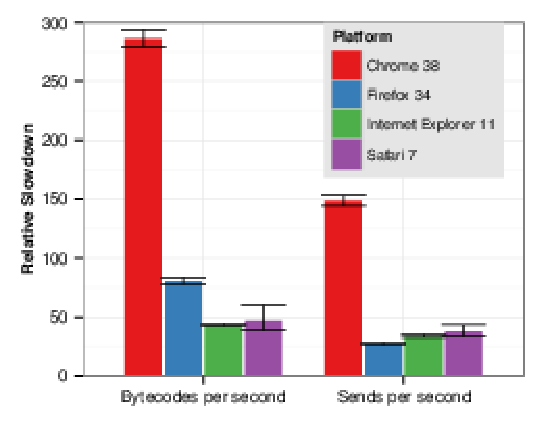
\includegraphics{benchmarks-speed}
  \caption[Slowdown Normalized to Squeak]{Overall speed: Bytecodes per second,
    sends per second. Each bar shows the arithmetic mean of 5 runs, normalized
    to the Squeak 3.9 interpreter \protect\acs{VM}. }
  \label{fig:results2}
\end{figure}

\subsection{Performance}
\label{sec:performance}

To measure the performance of \SqueakJS in various scenarios, we used
five benchmarks across Chrome 38, Firefox 34, Internet Explorer 11,
Squeak VM 3.9, and Safari 7. We used an older version of the Squeak
\ac{VM}, because newer versions cannot load the Squeak mini image we
used for testing. Our benchmarks are as follows:
\begin{description}
\item[blt] measures the efficiency of the BitBlt implementation. It
  renders alternating patterns of pixels to a bitmap, without drawing
  it to the screen.
\item[draw] measures how fast the \ac{VM} can push
  updates the the screen. A Mandala is drawn repeatedly and flushed to
  the display.
\item[fib] measures the impact of large stack depths
  and many sends by calculating Fibonacci numbers recursively.
\item[fill] measures the performance when allocating a large object
  and filling it with constant data.
\item[prims] measures raw bytecode performance by finding primes
  in a loop using a prime sieve.
\item[richards] measures allocation and send performance by simulating
  an operating system kernel.
\end{description}
Timing results of these benchmarks are presented in
\autoref{fig:results}. To make our measurements comparable, we report
the arithmetic mean of five benchmark runs along with
bootstrapped~\cite{davison+:1997:bootstrap-methods} confidence
intervals showing the \SI{95}{\percent} confidence level. The raw
numbers for these browsers as well as those of Squeak 3.9 and
Potato/JSqueak are included in the appendix (\autoref{tab:osx} and
\autoref{tab:win}).

A method, \lstinline|tinyBenchmarks|, is included in Squeak to measure
raw speed of sends and bytecode processing. It is used by various
\acp{VM} to give an indication of the number of bytecodes and sends
per second. Inverse speedup (\ie slowdown) in bytecodes per second
and sends per second is given in \autoref{fig:results2}.

These results show that \SqueakJS is, depending on the browser,
consistently between one and two orders of magnitude slower than the
Squeak Interpreter in C. Note also that these numbers do not change
significantly if we disable breaking out of the \ac{VM} to process
browser events or run them on the headless V8 \ac{VM}.

We have not spent time optimizing the \JS code because using \SqueakJS
already feels responsive. We already regard these performance results
as acceptable, but also see much room for optimization. For example,
we are planning to add a just-in-time compilation to \JS.

\begin{figure*}
  \centering
  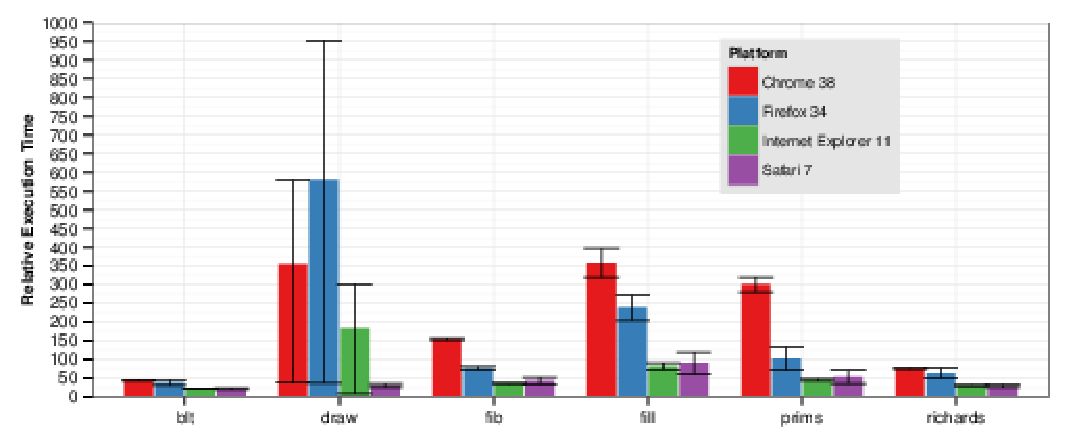
\includegraphics{benchmarks-timings}
  \caption[Benchmarks Normalized to Squeak]{Benchmark execution time results. 
Each bar shows the arithmetic mean of 5 runs, normalized to the Squeak 3.9
interpreter \protect\acs{VM}.  }
  \label{fig:results}
\end{figure*}

\section{Related Work}
\label{sec:related}

\paragraph{Squeak \protect\aclp{VM}}
\label{sec:squeakvms}

The root for all Squeak implementations is the original Squeak
\ac{VM}~\cite{IngallsKaehlerMaloneyWallaceKay97}, that aims to provide
an open Smalltalk-80 system~\cite{GoldbergRobson83}. Initially, the
original \ac{VM} did only provide an interpreter-based execution,
hence it is sometimes called \emph{interpreter} \ac{VM}; it serves as
the reference implementation for other Squeak \acp{VM}. A
\emph{Squeak Web Plugin} based on this \ac{VM} has been available for
several years; however, the plugin runs completely isolated from the
browser, thus, not providing any interaction from within the browser,
let alone \JS.

Another well-known Squeak \ac{VM} is the
Cog\ac{VM}~\cite{Miranda2011:The-Cog-Smalltalk-Virtual-Machine:},
providing a fully functional \ac{JIT} compiler for Squeak. Cog's
primary concern is performance.  Both are written in
\emph{Slang}~\cite{GuzdialRose02}, a Smalltalk subset that directly
translates to C.

The RoarVM~\cite{Ungar+2009:Hosting-an-object-heap} implements Squeak
with a focus on exploiting manycore hardware. It is written directly
in C++.

Potato\footnote{\url{http://sourceforge.net/projects/potatovm/}} and
its ancestor {JSqueak} are implementations of Squeak in Java.
\RSqueakVM, based on
Spy~\cite{Bolz+2008:Back-to-the-Future-in-One-Week}, is an
implementation of Squeak in the PyPy framework~\cite{Wassermann13}. It
is implemented in a subset of Python, RPython, to test its viability
as \ac{VM} platform.

NaClSqueak%
\footnote{\url{https://github.com/yoshikiohshima/NaClSqueak/}} is a
deviation of the Squeak \emph{interpreter} \ac{VM}, modified to run
natively on the NativeClient framework of the Chrome browser family.
Emscripten provides a similar option to NaCl, compiling C code
directly into \JS. While to the best of our knowledge there is no
Squeak \ac{VM} compiled with Emscripten, PyPy (which is based on the
same RPython translation toolchain that \RSqueakVM uses) has been
successfully compiled using Emscripten, and the same might work for
\RSqueakVM also. However, both NaCl and Emscripten focus on
whole-system translation, implement a C semantics, and are not
intended for rich interactions with the \JS environment. In this
regard, NaClSqueak and a hypothetical Emscripten-compiled Squeak
\ac{VM} come close to the Squeak Web Plugin. Their most direct
advantage is near native performance through highly optimized \JS
code, but they are difficult to debug and instrument from \JS.
Additionally, NativeClient is only available to Chrome browsers.

\paragraph{Dynamic languages on dynamic languages}
\label{sec:dynam-lang-impl}

Squeak itself can be run on top of Squeak within its
\emph{Simulator}. While being slow, this provides means of
introspection into the Squeak \ac{VM}. However, these means are
limited to the C-oriented view of Slang; objects of the hosted Squeak
image cannot be accessed as such. In \SqueakJS, objects of the hosted
Squeak are readily available.

Since Self 4.0, a Smalltalk
implementation~\cite{wolczko:1996:self-includes:} is an optional part
of the Self distribution. Here, Smalltalk is directly translated to
Self bytecode, without loss of expressiveness; there is no difference
between running Smalltalk code and running Self code in ``self
includes: Smalltalk''.

Amber\footnote{\url{http://amber-lang.net/}} is a Smalltalk dialect
implemented in \JS. It includes a complete development environment and
a Smalltalk-to-\JS compiler. Amber does not interpret bytecodes but
parses Smalltalk source code. Hence, it is not possible to load
pre-exisiting Squeak image files. The performance of Amber is in the
same order of magnitude as \SqueakJS. It is possible to directly call
\JS from Amber Smalltalk code.

Hobbes by Bykov is a \ac{VM} for the original Smalltalk-80 written in
VisualWorks Smalltalk and later ported by Ingalls to \SqueakST.

Whalesong~\cite{YooKrishnamurthi13} (Racket),
Biwa\footnote{\url{http://www.biwascheme.org/}} (Scheme), and
Skulpt\footnote{\url{https://github.com/skulpt/skulpt/}} (Python),
among others, are \JS implementations of \acp{VM} for dynamic
languages.

\paragraph{Other languages on top of \JS}
\label{sec:other-lang-ontop}

O'Browser~\cite{canou+:2008:obrowser:-objective} (OCaml),
BicaVM\footnote{\url{https://github.com/nurv/BicaVM/}} (Java), and
Doppio\footnote{\url{http://int3.github.io/doppio/about.html}} (Java), among
others, are \JS implementations of \acp{VM} for static languages.

For a plethora of languages, including Dart, CoffeeScript, TypeScript,
the Google Web Toolkit (Java) and others, source-to-source compilers
exists that emit \JS code as result of the compilation
process. Browsers then execute \JS, rather than the code of the source
language directly.

\section{Conclusion and Future Work}
\label{sec:conclusion}

We have presented our experience with implementing \SqueakJS, a fully
compatible implementation of a Squeak \ac{VM} that runs in modern Web
browsers. We were able to develop \SqueakJS quickly using a rapid
prototyping approach to \ac{VM} development. We started from the
earlier Potato design, which was small enough to be a tractable
experiment, yet complete enough to be motivating. From Potato,
\SqueakJS inherits its mapping of Squeak objects to native \JS objects
that can be inspected and manipulated using other \JS tools. This
allowed us to take advantage of mature \JS tools for development and
debugging and made a Web-appropriate adaption of file and image-file
management possible.

We also designed and implemented a hybrid \ac{GC} scheme to allow for
Squeak object enumeration without a dedicated object table, while
delegating as much work as possible to the \JS \ac{GC}. \SqueakJS
rarely has to do manual garbage collection, and even then our
algorithm provides good performance, pausing only in our setup for
about\SI{300}{\ms} with a typical object memory of 300,000
objects.

We have found that the Squeak \ac{VM} approach to provide a virtual
environment without direct access to platform libraries was useful for
our implementation. The Squeak plugin interface that abstracts from
many platform-specific details was implementable even in the \JS
environment.

Some non-essential primitives have fallback code in Squeak, so they
can initially be skipped during the implementation, and only be added
as an optimization. This made implementing easier. It would have been
nice if all non-essential primitives had working fallback code in
image, so that implementing Squeak runtime support on new platform can
be carried out even faster.

There are different directions for future work. Firstly, we want to
make \SqueakJS feature-complete so it can be used as a drop-in
replacement for a regular Squeak \ac{VM}. Weak references and
finalization are still missing, as are many modules, \eg to allow
\SqueakJS to play sounds or perform network requests. Secondly, to
improve performance, we are planning to add a \ac{JIT} that compiles
Squeak methods to \JS. We will investigate separating event-processing
and bytecode interpretation; currently, the constant switching between
both imposes a performance trade-off. Another significant increase in
responsiveness would come from improving BitBlt performance. One idea
would be to run BitBlt in a separate process to utilize multiple
cores. It might also be possible to re-implement it using GPU
processing via WebGL. Lastly, we would like to package \SqueakJS in a
way to be easily used on any web page, transforming it from a novelty
to a serious tool. This also means improving compatibility with a
wider range of web browsers on both desktop and mobile platforms.

\SqueakJS is still a very young project, but already
performs well enough to be usable, and is complete enough to run both
old and modern Squeak images.

\bibliographystyle{abbrvnat}
{
\begin{thebibliography}{20}
\providecommand{\natexlab}[1]{#1}
\providecommand{\url}[1]{\texttt{#1}}
\expandafter\ifx\csname urlstyle\endcsname\relax
  \providecommand{\doi}[1]{doi: #1}\else
  \providecommand{\doi}{doi: \begingroup \urlstyle{rm}\Url}\fi

\bibitem[Bolz(2012)]{Bolz12}
C.~F. Bolz.
\newblock \emph{{Meta-tracing Just-in-time Compilation for RPython}}.
\newblock PhD thesis, Mathematisch-Naturwissenschaftliche Fakult\"at, Heinrich
  Heine Universit\"at D\"usseldorf, 2012.

\bibitem[Bolz et~al.(2008)Bolz, Kuhn, Lienhard, Matsakis, Nierstrasz, Renggli,
  Rigo, and Verwaest]{Bolz+2008:Back-to-the-Future-in-One-Week}
C.~F. Bolz, A.~Kuhn, A.~Lienhard, N.~D. Matsakis, O.~Nierstrasz, L.~Renggli,
  A.~Rigo, and T.~Verwaest.
\newblock {Back to the Future in One Week---Implementing a Smalltalk VM in
  PyPy}.
\newblock In \emph{Self-Sustaining Systems (S3)}, volume 5146 of \emph{Lecture
  Notes in Computer Science}, pages 123--139. Springer, 2008.

\bibitem[Canou et~al.(2008)Canou, Balat, and
  Chailloux]{canou+:2008:obrowser:-objective}
B.~Canou, V.~Balat, and E.~Chailloux.
\newblock {O'Browser: Objective Caml on Browsers}.
\newblock In \emph{ACM SIGPLAN Workshop on ML}, pages 69--78. ACM, 2008.

\bibitem[Davison and Hinkley(1997)]{davison+:1997:bootstrap-methods}
A.~C. Davison and D.~V. Hinkley.
\newblock \emph{Bootstrap Methods and Their Application}, chapter~5.
\newblock Cambridge, 1997.

\bibitem[Goldberg and Robson(1983)]{GoldbergRobson83}
A.~Goldberg and D.~Robson.
\newblock \emph{{Smalltalk-80: The Language and its Implementation}}.
\newblock Addison-Wesley, 1983.

\bibitem[Guzdial and Rose(2002)]{GuzdialRose02}
M.~Guzdial and K.~Rose.
\newblock \emph{{Squeak---Open Personal Computing and Multimedia}}.
\newblock Prentice Hall, 2002.

\bibitem[Hickson(2013)]{hickson2013web}
I.~Hickson.
\newblock Web storage.
\newblock \emph{W3C Recommendation}, 2013.

\bibitem[Ingalls et~al.(1997)Ingalls, Kaehler, Maloney, Wallace, and
  Kay]{IngallsKaehlerMaloneyWallaceKay97}
D.~H. Ingalls, T.~Kaehler, J.~Maloney, S.~Wallace, and A.~Kay.
\newblock {Back to the Future: the Story of Squeak, a Practical Smalltalk
  Written in Itself}.
\newblock In \emph{Conference on Object- Oriented Programming, Systems,
  Languages, and Applications (OOPSLA)}, pages 318--326. ACM, 1997.

\bibitem[Kay(2005)]{Kay05}
A.~Kay.
\newblock {Squeak Etoys, Children \& Learning}.
\newblock Technical Report RN-2005-001, Viewpoints Research Institute, 2005.

\bibitem[Lincke et~al.(2012)Lincke, Krahn, Ingalls, R\"oder, and
  Hirschfeld]{lincke2012lively}
J.~Lincke, R.~Krahn, D.~Ingalls, M.~R\"oder, and R.~Hirschfeld.
\newblock {The Lively PartsBin: A Cloud-Based Repository for Collaborative
  Development of Active Web Content}.
\newblock In \emph{Hawaii International Conference on System Science (HICSS)},
  pages 693--701. IEEE, 2012.

\bibitem[Maloney(1995)]{maloney1995morphic}
J.~Maloney.
\newblock Morphic: The self user interface framework.
\newblock \emph{Self}, 4, 1995.

\bibitem[Maloney et~al.(2004)Maloney, Burd, Kafai, Rusk, Silverman, and
  Resnick]{maloney2004scratch}
J.~Maloney, L.~Burd, Y.~Kafai, N.~Rusk, B.~Silverman, and M.~Resnick.
\newblock {Scratch: A Sneak Preview}.
\newblock In \emph{Conference on Creating, Connecting and Collaborating through
  Computing (C5)}, pages 104--109. IEEE, 2004.

\bibitem[Marr and D'Hondt(2012)]{marr2012identifying}
S.~Marr and T.~D'Hondt.
\newblock {Identifying a Unifying Mechanism for the Implementation of
  Concurrency Abstractions on Multi-language Virtual Machines}.
\newblock In \emph{Conference on Objects, Models, Components, Patterns
  (TOOLS)}, volume 7304 of \emph{Lecture Notes in Computer Science}, pages
  171--186. Springer, 2012.

\bibitem[Mehta et~al.(2013)Mehta, Sicking, Graff, Popescu, Orlow, and
  Bell]{mehta2013indexed}
N.~Mehta, J.~Sicking, E.~Graff, A.~Popescu, J.~Orlow, and J.~Bell.
\newblock Web storage.
\newblock \emph{W3C Candidate Recommendation}, 2013.

\bibitem[Miranda(2011)]{Miranda2011:The-Cog-Smalltalk-Virtual-Machine:}
E.~Miranda.
\newblock {The Cog Smalltalk Virtual Machine: Writing a JIT in a High-level
  Dynamic Language}.
\newblock In \emph{Workshop on Virtual Machines and Intermediate Languages
  (VMIL)}, 2011.

\bibitem[Ungar and Adams(2009)]{Ungar+2009:Hosting-an-object-heap}
D.~Ungar and S.~S. Adams.
\newblock {Hosting an Object Heap on Manycore Hardware: an Exploration}.
\newblock \emph{SIGPLAN Notices}, 44\penalty0 (12):\penalty0 99--110, 2009.

\bibitem[Wassermann(2013)]{Wassermann13}
L.~Wassermann.
\newblock {Tracing Algorithmic Primitives in R/Squeak-VM}.
\newblock Master's thesis, Software Architecture Group, Hasso-Plattner-Institut
  Potsdam, 2013.

\bibitem[Wolczko(1996)]{wolczko:1996:self-includes:}
M.~Wolczko.
\newblock {self includes: Smalltalk}.
\newblock In \emph{Workshop on Prototype-Based Languages (co-located with
  ECOOP), Linz, Austria}, 1996.

\bibitem[Yoo and Krishnamurthi(2013)]{YooKrishnamurthi13}
D.~Yoo and S.~Krishnamurthi.
\newblock {Whalesong: Running Racket in the Browser}.
\newblock \emph{SIGPLAN Notices}, 49\penalty0 (2):\penalty0 97--108, 2013.

\bibitem[Zakai(2011)]{Zakai11}
A.~Zakai.
\newblock {Emscripten: An LLVM-to-JavaScript Compiler}.
\newblock In \emph{SPLASH'11 Companion (Wavefront)}, pages 301--312. ACM, 2011.

\end{thebibliography}

}

\clearpage
\appendix
\null

\section*{Appendix}
\label{sec:appendix}
\begingroup
\renewcommand*\thetable{\Alph{table}}
\setcounter{table}{0}
\itshape

For reference, we present the raw data for our benchmarks in
\autoref{tab:win} and \autoref{tab:osx}. Due to operating system
restrictions, it was impossible to run all Squeak platforms on the
same machine. Therefore, the numbers for Safari are normalized to
Squeak on OS\,X while all numbers of the other platforms are
normalized to Squeak on Windows.

\autoref{tab:platforms} lists all exact version numbers of the
platforms used.

\begin{table}[h]
  \centering
   % benchmarks-platforms
{\footnotesize
\begin{tabular}{ll}
\toprule
\multicolumn{1}{l}{ }&\multicolumn{1}{c}{Full version}\tabularnewline
\midrule
Squeak 3.9&SqueakVM 3.9\tabularnewline
Potato 0.1&Potato (formerly JSqueak) 0.1\tabularnewline
Firefox 34&Firefox 34.0a1 (2014-07-23)\tabularnewline
Chrome 38&Chrome 38.0.2002.0\tabularnewline
Internet Explorer 11&Internet Explorer 11.0.9600.17207\tabularnewline
SqueakOSX&Squeak 4.2.5beta1U\tabularnewline
Safari 7&Safari 7.0.5 (9537.77.4)\tabularnewline
\bottomrule
\end{tabular}}

  \caption{Exact platform versions}
  \label{tab:platforms}
\end{table}
\begin{table}[h]
 \centering
   % benchmarks-osx-timings
{\footnotesize
\begin{tabular}{lr@{\,\si{\milli\second} \ensuremath{\pm}}rcr@{\,\si{\milli\second} \ensuremath{\pm}}r}
\toprule
\multicolumn{1}{l}{\bfseries Benchmark}&\multicolumn{2}{c}{\bfseries Safari 7}&\multicolumn{1}{c}{\bfseries }&\multicolumn{2}{c}{\bfseries SqueakOSX}\tabularnewline
\cline{2-3} \cline{5-6}
\multicolumn{1}{l}{}&\multicolumn{1}{c}{mean}&\multicolumn{1}{c}{error}&\multicolumn{1}{c}{}&\multicolumn{1}{c}{mean}&\multicolumn{1}{c}{error}\tabularnewline
\midrule
blt&$ 539.600$&$ 46.126$&&$ 24.000$&$1.640$\tabularnewline
draw&$1251.600$&$126.036$&&$ 40.200$&$5.660$\tabularnewline
fib&$ 790.200$&$175.777$&&$ 18.200$&$0.392$\tabularnewline
fill&$ 254.000$&$ 81.655$&&$  2.800$&$0.392$\tabularnewline
prims&$ 266.400$&$ 99.794$&&$  5.000$&$0.000$\tabularnewline
richards&$5393.000$&$757.060$&&$185.200$&$3.124$\tabularnewline
\bottomrule
\end{tabular}}
\\
   % benchmarks-osx-speed
{\footnotesize
\begin{tabular}{lrrcrr}
\toprule
\multicolumn{1}{l}{\bfseries  }&\multicolumn{2}{c}{\bfseries Safari 7}&\multicolumn{1}{c}{\bfseries }&\multicolumn{2}{c}{\bfseries SqueakOSX}\tabularnewline
\cline{2-3} \cline{5-6}
\multicolumn{1}{l}{}&\multicolumn{1}{c}{mean}&\multicolumn{1}{c}{error}&\multicolumn{1}{c}{}&\multicolumn{1}{c}{mean}&\multicolumn{1}{c}{error}\tabularnewline
\midrule
Bytecodes&$16655888$&$4051326$&&$782878362$&$13360834$\tabularnewline
Sends&$  565604$&$  82545$&&$ 21313809$&$  490523$\tabularnewline
\bottomrule
\end{tabular}}

  \caption{Benchmarks and speeds, raw numbers (run on OS\,X on Intel Core
    i7-4850HQ CPU @ 2.30 GHz) }
  \label{tab:osx}
\end{table}

\begin{sidewaystable}
  \centering
   % benchmarks-timings
{\footnotesize
\begin{tabular}{lr@{\,\si{\milli\second} \ensuremath{\pm}}rcr@{\,\si{\milli\second} \ensuremath{\pm}}rcr@{\,\si{\milli\second} \ensuremath{\pm}}rcr@{\,\si{\milli\second} \ensuremath{\pm}}rcr@{\,\si{\milli\second} \ensuremath{\pm}}r}
\toprule
\multicolumn{1}{l}{\bfseries Benchmark}&\multicolumn{2}{c}{\bfseries Chrome 38}&\multicolumn{1}{c}{\bfseries }&\multicolumn{2}{c}{\bfseries Firefox 34}&\multicolumn{1}{c}{\bfseries }&\multicolumn{2}{c}{\bfseries Internet Explorer 11}&\multicolumn{1}{c}{\bfseries }&\multicolumn{2}{c}{\bfseries Potato 0.1}&\multicolumn{1}{c}{\bfseries }&\multicolumn{2}{c}{\bfseries Squeak 3.9}\tabularnewline
\cline{2-3} \cline{5-6} \cline{8-9} \cline{11-12} \cline{14-15}
\multicolumn{1}{l}{}&\multicolumn{1}{c}{mean}&\multicolumn{1}{c}{error}&\multicolumn{1}{c}{}&\multicolumn{1}{c}{mean}&\multicolumn{1}{c}{error}&\multicolumn{1}{c}{}&\multicolumn{1}{c}{mean}&\multicolumn{1}{c}{error}&\multicolumn{1}{c}{}&\multicolumn{1}{c}{mean}&\multicolumn{1}{c}{error}&\multicolumn{1}{c}{}&\multicolumn{1}{c}{mean}&\multicolumn{1}{c}{error}\tabularnewline
\midrule
blt&$ 1121.800$&$ 19.584$&&$  982.800$&$ 188.140$&&$ 564.000$&$ 8.129$&&$ 252.400$&$  19.418$&&$ 25.800$&$0.733$\tabularnewline
draw&$ 3337.800$&$ 86.112$&&$ 5451.600$&$  44.438$&&$1717.400$&$51.153$&&$   0.000$&$   0.000$&&$  9.400$&$7.244$\tabularnewline
fib&$ 2912.000$&$ 16.883$&&$ 1448.400$&$  82.329$&&$ 671.000$&$ 7.094$&&$ 150.200$&$   5.382$&&$ 18.800$&$0.392$\tabularnewline
fill&$ 1147.400$&$ 18.988$&&$  765.000$&$  72.171$&&$ 263.800$&$ 2.659$&&$5201.400$&$  82.381$&&$  3.200$&$0.392$\tabularnewline
prims&$ 1745.000$&$ 22.079$&&$  594.600$&$ 198.044$&&$ 263.800$&$ 1.143$&&$ 391.800$&$ 408.781$&&$  5.800$&$0.392$\tabularnewline
richards&$13816.400$&$116.125$&&$11684.000$&$2844.545$&&$5643.000$&$45.448$&&$8249.000$&$6761.833$&&$182.600$&$3.136$\tabularnewline
\bottomrule
\end{tabular}}
\\
   % benchmarks-speed
{\footnotesize
\begin{tabular}{lrrcrrcrrcrrcrr}
\toprule
\multicolumn{1}{l}{\bfseries  }&\multicolumn{2}{c}{\bfseries Chrome 38}&\multicolumn{1}{c}{\bfseries }&\multicolumn{2}{c}{\bfseries Firefox 34}&\multicolumn{1}{c}{\bfseries }&\multicolumn{2}{c}{\bfseries Internet Explorer 11}&\multicolumn{1}{c}{\bfseries }&\multicolumn{2}{c}{\bfseries Potato 0.1}&\multicolumn{1}{c}{\bfseries }&\multicolumn{2}{c}{\bfseries Squeak 3.9}\tabularnewline
\cline{2-3} \cline{5-6} \cline{8-9} \cline{11-12} \cline{14-15}
\multicolumn{1}{l}{}&\multicolumn{1}{c}{mean}&\multicolumn{1}{c}{error}&\multicolumn{1}{c}{}&\multicolumn{1}{c}{mean}&\multicolumn{1}{c}{error}&\multicolumn{1}{c}{}&\multicolumn{1}{c}{mean}&\multicolumn{1}{c}{error}&\multicolumn{1}{c}{}&\multicolumn{1}{c}{mean}&\multicolumn{1}{c}{error}&\multicolumn{1}{c}{}&\multicolumn{1}{c}{mean}&\multicolumn{1}{c}{error}\tabularnewline
\midrule
Bytecodes&$2296769$&$8200$&&$8186019$&$214742$&&$15157722$&$82399$&&$22126742$&$245474$&&$657239930$&$17551026$\tabularnewline
Sends&$ 135157$&$ 625$&&$ 737809$&$ 19835$&&$  591498$&$ 1307$&&$ 2685416$&$ 62465$&&$ 20096527$&$  702311$\tabularnewline
\bottomrule
\end{tabular}}

  \caption{Benchmarks and speeds, raw numbers (run on Windows on Intel
    Core i5-4300U CPU @ 2.80 GHz). Note that Potato could not run the
    \textbf{draw} benchmark due to its incomplete BitBlt
    implementation, and that the \textbf{fill} and \textbf{richards}
    benchmarks, both of which put much pressure on the GC, perform
    very badly on Potato.}
  \label{tab:win}
\end{sidewaystable}

\endgroup
\end{document}

%%% Local Variables:
%%% mode: latex
%%% TeX-master: t
%%% End:
